\documentclass[../../main.tex]{subfiles}
% \graphicspath{{\subfix{../images/}}}

\begin{document}
Las Redes Neuronales Recurrentes (RNR) son una familia de redes neuronales pensadas
específicamente para trabajar con \textbf{datos secuenciales} en donde el orden importa.
Es por esto que han sido y continúan siendo muy útiles en tareas como análisis de series
temporales y procesamiento de lenguaje natural.

A diferencia de las redes feedforward como las que venimos presentando hasta el momento,
en donde la información fluye solamente en una dirección, pasando de las neuronas de una
capa a las de la capa siguiente, lo que caracteriza a las RNR es la presencia de cíclos en
su grafo. Estos cíclos hacen que las neuronas de la red puedan tomar como entradas
sus propias salidas de pasos anteriores, permitiéndole a la red de esta forma tener
un \textbf{estado interno} o \textbf{memoria}: entradas recibidas en pasos más empranos
afectan la respuesta de la red ante la entrada actual \cite{ai-a-modern-approach}.

Para comprender un poco más este comportamiento, tomemos la más simple de las RNR,
compuesta por una única neurona (oculta) que recibe la entrada correspondiente al tiempo
\(t\), produce una salida y se la envía a sí misma \cite{hands-on-ML-sklearn-tf}, como se
puede ver a la izquierda del Diagrama \ref{fig:simple-rnn}. Así, en cada paso \(t\), la
\textit{neurona ``recurrente''} recibe no solo la entrada \(x_t\) sino también su propia
salida computada en el paso anterior, \(y_{t-1}\). Esto se hace aún más evidente cuando
``desenrollamos'' la red a lo largo del tiempo, cuya representación se encuentra a la
derecha de la Figura \ref{fig:simple-rnn} y se asemeja a la de una feedforward.

\begin{figure}[h]
    \centering
    \begin{tikzpicture}[
        item/.style={circle,draw,thick,align=center},
        itemc/.style={item,on chain,join}
    ]
    % Unenrolled RNN (on the right)
        \begin{scope}[
            start chain=going right,
            nodes=itemc,
            every join/.style={-latex,very thick},
            node distance=3em,
            local bounding box=chain
        ]
        \path
            node (f0) {\(f\)}
            node (f1) {\(f\)}
            node (f2) {\(f\)}
            node[xshift=2em] (ft) {\(f\)};
        \end{scope}
        \foreach \i/\j in {0/1, 1/2, 2/t} {
            \draw[very thick,-latex]
                (f\i) -- node[pos=0.4,fill=white] {\scriptsize \(w_{f,f}\)} (f\j);
        }

        \foreach \X in {0,1,2,t}{
            \draw[very thick,-latex] (f\X.north) -- ++ (0, 3.5em)
                node[above,item,fill=gray!10] (y\X) {\(y_\X\)}
                node[pos=0.4,fill=white] {\footnotesize\shortstack{\(w_{0_f, y}\)\\\(w_{f, y}\)}};
            \draw[very thick,latex-] (f\X.south) -- ++ (0, -3.5em)
                node[below,item,fill=gray!10] (x\X) {\(x_\X\)}
                node[pos=0.6,fill=white] {\footnotesize\shortstack{\(w_{0_x, f}\)\\\(w_{x, f}\)}};
        }
        \path (x2) -- (xt) node[midway,scale=2,font=\bfseries] {\dots};

        % Equal sign
        \node[left=1em of chain,scale=2] (eq) {\(=\)};

        % Folded RNN (on the left)
        \node[left=2em of eq,item] (f) {\(f\)};
        \path (f) edge[
            out=135, in=225, looseness=5, ->, very thick
        ] node[pos=0.5,fill=white] {\scriptsize \(w_{f,f}\)} (f);
        \draw[very thick,-latex]
            (f.north) -- ++ (0, 3.5em)
            node[above,item,fill=gray!10] {\(y_t\)}
            node[pos=0.4,fill=white] {\footnotesize\shortstack{\(w_{0_f,y}\)\\\(w_{f, y}\)}};
        \draw[very thick,latex-]
            (f.south) -- ++ (0, -3.5em)
            node[below,item,fill=gray!10] {\(x_t\)}
            node[pos=0.6,fill=white] {\footnotesize\shortstack{\(w_{0_x,f}\)\\\(w_{x, f}\)}};
    \end{tikzpicture}
    \caption{A la izquierda, se ve la más simple de las Redes Neuronales Recurrentes, con
    solamente la capa de entrada, una capa oculta formada por una neurona con su
    respectiva conexión recurrente, y la capa de salida. A la derecha, se ve la misma red
    pero ``desenrollada'' a lo largo del tiempo. Asumiremos por simplicidad que tanto la
    entrada como la salida en cada momento \(t\) son simplemente números real, es decir
    \(x_t, y_t \in \mathbb{R} \ \forall t\). Denotamos con \(w_{x,f}\) al peso que va
    desde la entrada a la neurona oculta, con \(w_{0_x,f}\) al asociado a la neurona dummy
    con valor fijo en 1 que está en la entrada, con \(w_{f,y}\) al que va desde la neurona
    oculta hasta la capa de salida, con \(w_{0_f, y}\) al bias entre la oculta y la de
    salida, y con \(w_{f,f}\) al peso que aplica la neurona sobre su propia salida del paso
    anterior.}
    \label{fig:simple-rnn}
\end{figure}

Cada neurona realiza lo mismo que en una red feeforward, en el sentido que computan una
suma pesada de sus entradas y aplican una función de activación sobre esta. Sin embargo, a
partir de la Figura \ref{fig:simple-rnn}, podemos notar dos particularidades con respecto
a las redes recurrentes: \vspace{-0.25cm}
\begin{itemize}[itemsep=0.1cm]
    \item Por un lado, cada neurona tiene un peso extra además del que se aplica sobre la
    entrada \(x_t\), el cual está denotado en la Figura con \(w_{x,f}\). Este peso extra
    corresponde al que se aplica sobre la salida de la neurona en el paso anterior
    \(f_{t-1}\), denotado con \(w_{f,f}\).
    \item Por otro lado, la red utiliza los mismos pesos \(w_{x,f}\), \(w_{f,f}\) y
    \(w_{f,y}\) en \textit{todos} los pasos de tiempo.
\end{itemize}

Con esto en cuenta, vamos a tener que el cómputo llevado a cabo por la red
en cada paso de tiempo \(t\) está dado por:
\begin{align*}
    f_t &=\ a_f \left( w_{x,f} x_t  + w_{f,f} f_{t-1} + w_{0,f} \right) \\
    y_t &=\ a_y \left( w_{f,y} f_t + w_{0,y} \right) \\
\end{align*}
donde \(a_f\) denota la función de activación seleccionada para la capa oculta y \(a_y\)
la de la capa de salida. Algo que vale la pena aclarar es que para el primer paso
de tiempo, lo que sería la salida del paso anterior se establace manualmente, como
por ejemplo con el valor 0.

Nos concentremos en la salida de la neurona recurrente en el tiempo \(t\), es decir
en \(f_t\), dejando la salida de la red \(y_t\) de lado. A partir de las Ecuaciones
anteriores, podemos ver lo que venimos explicando: \(f_t\) es una función de
tanto la entrada en el tiempo actual \(x_t\) y de su salida en el paso anterior
\(f_{t-1}\). Entonces, si tomamos un \(t' > 0\) fijo, vamos a tener que:
\begin{itemize}[itemsep=0.05cm]
    \item \(f_{t'}\) es una función de \(x_{t'}\) y de \(f_{t'-1}\), pero
    \item \(f_{t'-1}\) es a su vez una función de \(x_{t'-1}\) y de \(f_{t'-2}\), pero
    \item \(f_{t'-2}\) es a su vez una función de \(x_{t'-2}\) y de \(f_{t'-3}\),
    \item y así sucesivamente
\end{itemize}
Este comportamiento hace que \(f_{t'}\) sea una función de todas las entradas vistas desde
\(t=0\), constituyendo de esta forma una especie \textit{memoria}, que se suele llamar
\textbf{estado oculto} de la neurona. En este caso, como la red solamente tiene una capa
oculta con una neurona recurrente, el estado oculto de la neurona coincide con el estado
oculto de la red.

De la misma forma en que lo hicimos anteriormente para las redes feedforward, podemos
empezar a complejizar esta red agregando varias neuronas recurrentes en la capa oculta,
cada una con su propio ciclo, como se puede ver en la Figura \ref{fig:simple-rnn-2}.
\begin{figure}[h]
    \centering
    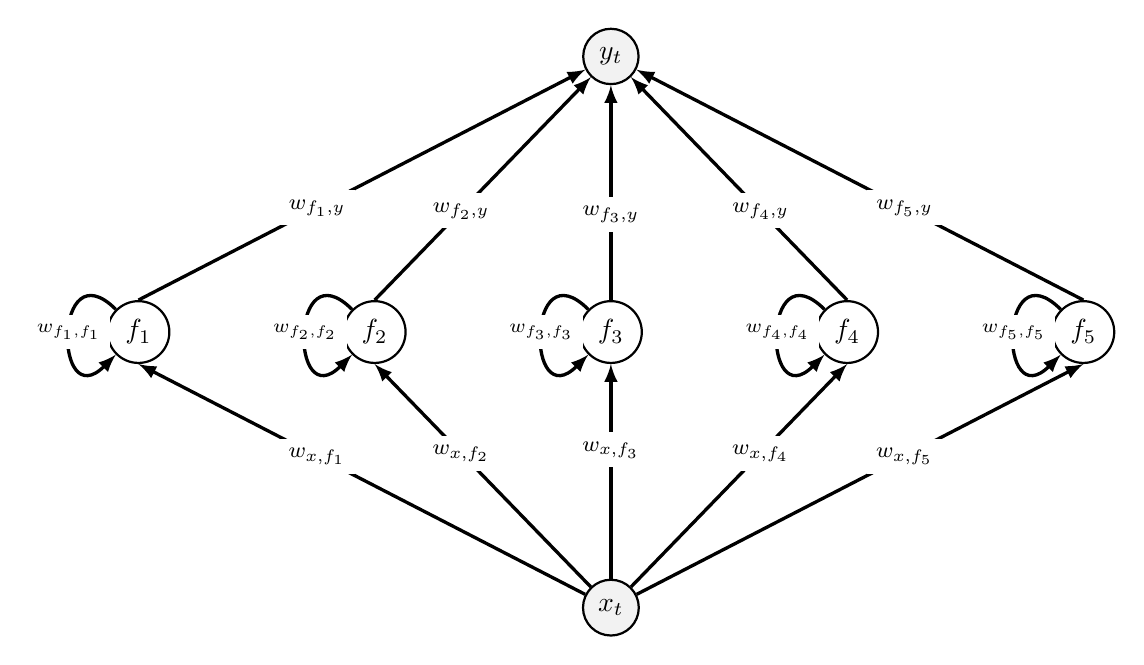
\begin{tikzpicture}[
        item/.style={circle, draw, thick, align=center, minimum size=2em},
        >=latex
    ]
    \def\n{5}    % number of recurrent neurons
    \def\xsep{3} % horizontal separation in em

    \node[item, fill=gray!10] (x) at ({(\n-1)*\xsep/2}, -3.5) {\(x_t\)};
    \node[item, fill=gray!10] (y) at ({(\n-1)*\xsep/2}, 3.5) {\(y_t\)};

    % Loop through to create f_i nodes
    \foreach \i in {1,...,\n} {
        \pgfmathsetmacro{\x}{(\i-1)*\xsep}
        \node[item] (f\i) at (\x, 0) {\(f_{\i}\)};

        % Arrow up to y_t
        \draw[very thick,-latex]
            (f\i.north) -- (y)
            node[pos=0.4,fill=white] {\footnotesize{\(w_{f_\i, y}\)}};

        % Self-loop
        \path (f\i) edge[out=135, in=225, looseness=5, ->, very thick]
            node[pos=0.5,fill=white] {\scriptsize \(w_{f_\i,f_\i}\)} (f\i);
        % Arrow down from x_t
        \draw[very thick,latex-]
            (f\i.south) -- (x)
            node[pos=0.4,fill=white] {\footnotesize{\(w_{x, f_\i}\)}};
    }
    \end{tikzpicture}
    \caption{Red Neuronal Recurrente con una capa oculta de 5 neuronas recurrentes,
    cada una con su ciclo. Similarmente al Diagrama anterior, denotamos con ...
    \textbf{TODO}}
    \label{fig:simple-rnn-2}
\end{figure}

Con esto, vamos a tener que el estado oculto de la red va a ser un vector formado por el
estado oculto de las 5 neuronas. O sea, si denotamos con \(f_t\) al estado oculto
de la red en el tiempo \(t\) y con \(f_{i_t}\) al estado oculto de la neurona oculta
\(i\), en el tiempo \(t\) vamos a tener que:
\begin{equation*}
    f_t = (f_{1_t}, f_{2_t}, f_{3_t}, f_{4_t}, f_{5_t})
\end{equation*}

Y también podemos volver a utilizar la notación matricial para describir el comportamiento
de la red:
\begin{align*}
    f_t &=\ \bm{a}_t \left( \mathbf{W}_x x^T + \mathbf{W}_f f_{t-1}^T \right) \\
    y_t &=\ \bm{a}_y \left( \mathbf{W}_y f_t \right)
\end{align*}
donde:
\begin{itemize}[itemsep=0.05cm]
    \item \(\bm{a}_t\) es la función de activación de la capa oculta, aplicada elemento a
    elemento, es decir \(\bm{a}_t(x_0, x_1, ..., x_n) = (a_t(x_0), a_t(x_1), ...,
    a_t(x_n))\).
    \item \(\mathbf{W}_x\) es la matriz de tamaño \(k \times (n+1)\) de pesos que salen
    desde la capa de entrada hasta la capa oculta, incluyendo el bias, donde \(k\) es el
    número de neuronas en la capa oculta y \(n\) el tamaño de la entrada.
    \item \(x^T\) es el vector transpuesto de la entrada, junto con el 1 del bias.
    En este caso, estamos asumiendo \(x \in \mathbb{R}\).
    \item \(\mathbf{W}_f\) es la matriz diagonal de tamaño \(k \times k\) de pesos
    recurrentes. En cada elemento de la diagonal \(i\) se encuentra el peso que va desde
    la neurona \(i\) a sí misma, es decir \(w_{f_i, f_i}\).
    \item \(f_{t-1}^T\) es el estado oculto de la red en el paso de tiempo anterior.
    \item \(\bm{a}_y\) es la función de activación de la capa de salida, aplicada elemento a
    elemento, al igual que \(\bm{a}_t\).
    \item \(\mathbf{W}_y\) es la matriz de tamaño \(o \times (k+1)\) de pesos que van
    desde la capa oculta hasta la capa de salida, incluyendo el bias, donde \(o\) es el
    tamaño de la salida. En nuestra red, tomamos \(o=1\).
\end{itemize}

Al igual que antes, se pueden agregar más capas de neuronas recurrentes a la red,
permitiendo de esta manera que cada capa tenga su propio estado oculto. En este caso,
lo que va a ocurrir es que el estado oculto producido por las neuronas de una capa



\subsection{Long Short-Term Memory}

\subsection{Gated Recurrent Unit}

\end{document}